\documentclass[a4paper]{article}

\usepackage{style}

\begin{document}

    \copertina

    \tableofcontents

    \newpage

    \section{Introduzione}
	    In questa sezione vengono illustrate alcune informazioni utili per i valutatori. % anche vuoto
	    	\subsection{Abstract}
		    	Il progetto \textit{Adrenaline Motocross Park}, svolto per il corso di Tecnologie Web nell'anno accademico 2021-2022, propone di implementare un sito web adibito a facilitare la gestione delle prenotazioni dei servizi offerti dall'impianto sportivo ai clienti.

\textit{Adrenaline Motocross Park} è un impianto sportivo per la pratica del motocross, aperto ai piloti tra i 10 e 50 anni di età. È considerato uno degli impianti più all'avanguardia d'Italia, grazie alle sue numerose piste e all'alta qualità dei servizi offerti. I piloti possono usufruire di una vasta gamma di tracciati di diverse difficoltà, in modo tale da accontentare sia il neofita che il professionista. Vi è anche la possibilità di effettuare dei corsi di guida con istruttori professionali. Un altro punto di forza è sicuramente il noleggio delle moto e attrezzatura, un ottimo modo per offrire la possibilità a chi non conosce questo sport di provarlo. Oltre ai servizi fondamentali già elencati, l'impianto mette a disposizione dei clienti una serie di servizi accessori.

Vista l'importante affluenza di piloti all'interno dell'impianto e la conseguente difficoltà per la direzione di tenere traccia delle prenotazioni, i gestori hanno deciso di creare un sito web per la prenotazione di ingressi, corsi e noleggi. Si considera questa soluzione molto efficiente ed efficacie, in quanto può potenzialmente ridurre di molto le code all'ingresso, agevolando il lavoro degli amministratori e migliorando l'esperienza complessiva del cliente.

Per conseguire lo scopo stabilito, si è deciso di creare qualcosa di elegante ed efficace allo stesso tempo, in modo da garantire all'utente un'esperienza piacevole non solo in pista, ma anche online. Per i frequentatori del sito è possibile registrarsi e creare il proprio account personale, grazie al quale essi possono prenotare:
\begin{itemize}
\item Ingressi presso l'impianto;
\item Un posto per i corsi ai quali è interessato a partecipare;
\item Noleggio della moto in una data in cui ha prenotato un ingresso o un corso.
\end{itemize}

Oltre alla funzione prettamente gestionale, il sito deve offrire tutte le informazioni che possono essere d'interesse per il cliente:
\begin{itemize}
\item Tracciati: informazioni sul tracciato e orari di apertura;
\item Date di apertura: prossime date in cui l'impianto sarà aperto;
\item Corsi: prossimi corsi organizzati nell'impianto;
\item Servizi: gamma di servizi aggiuntivi offerti dall'impianto;
\item Contatti: recapiti dell'impianto.
\end{itemize}

	\newpage

	\section{Analisi}
		\input{Sezioni/Analisi/Analisi.tex} % anche vuoto
		\subsection{Studio dell'utenza finale}
			Il progetto \textit{Adrenaline Motocross Park} si propone come piattaforma di prenotazione per un parco divertimenti dedicato ai motociclisti
e agli appassionati di motocross. L'intervallo d'età si attesta tra i 12 e i 45 anni circa e, essendo comunque uno sport molto particolare,
il linguaggio sarà nella maggior parte semplice e più tecnico in alcuni tratti (pochi). Essendo pensata più come piattaforma di prenotazione
per i clienti dell'impianto, si presuppone che l'utenza conosca il linguaggio tecnico dello sport, ma abbiamo comunque pensato anche agli
utenti che si vogliono affacciare per la prima volta.
		\subsection{Possibili ricerche sui motori di ricerca}
			Vengono ora elencate, in ordine di rilevanza (dal particolare al generale), le ricerche che dovrebbero presentare il sito web tra i risultati.

%adrenaline motocross park
La query a cui sicuramente deve rispondere in primis il sito, è quella che contiene il nome stesso dell'impianto, \textit{Adrenaline Motocross Park}. Essendo l'impianto rinomato a livello nazionale e internazionale, il suo nome verrà spesso utilizzato nelle ricerche da parte dei piloti (per fama dell'impianto) e dei team (per livello e qualità dei servizi offerti).

%piste motocross
Dato il livello e il numero dei tracciati dell'impianto, è di fondamentale importanza che il sito risponda, in una ricerca, a tutte le query che contengono le parole \textit{piste, motocross, tracciati, piste minicross}. Questo tipo di ricerca è quella che viene maggiormente effettuata dai piloti, professionisti e amatoriali, nel momento in cui vogliono scoprire nuovi impianti in cui andare a correre.

%corsi motocross
È importante che il sito possa essere raggiunto anche da persone che vogliono affacciarsi a questo sport e da piloti neofiti. Per questo motivo il sito deve poter comparire anche nelle ricerche che contengono le parole \textit{corsi motocross, corsi di guida moto, come iniziare a fare motocross, ...} Un'obiettivo dell'impianto è quello di espandere la clientela, e rispondere a questa query è un potenziale modo per farlo.

%noleggio moto
L'impianto vuole anche poter sfruttare il servizio di noleggio per essere raggiunto. Alla luce di questo è interessante per i gestori fare in modo che il sito venga raggiunto anche da clienti occasionali, ovvero clienti che:
\begin{itemize}
\item Non praticano l'attività sportiva in modo continuativo e quindi non posseggono una moto;
\item Vogliono provare i nuovi modelli di moto usciti sul mercato;
\item Vogliono provare a praticare questo sport senza l'onere di prendere, nell'insicurezza, una moto e l'attrezzatura necessaria.
\end{itemize}

%motorsport
Un altro ambito, meno rilevante, di interesse dell'impianto è quello di attirare visitatori che assistano a gare e/o ad allenamenti. Affinché questo sia possibile, è bene che il sito possa essere raggiungibile anche dagli utenti che ricerchino eventi sportivi in generale. Il sito deve poter comparire in ricerche le cui parole chiave siano \textit{eventi sportivi nazionali, eventi sportivi Padova, eventi motociclistici}.

Oltre a questi principali casi in cui il sito deve comparire tra le ricerche, vi sono tutta una serie di parole chiave generali: \textit{sport Padova, sport estremi Padova, motocross veneto, ...}

Il target del sito è una nicchia molto ristretta, per questo si vuole premere particolarmente su ricerche specifiche del settore, essendo consapevoli che la barriera per l'accesso ad uno sport come il motocross è molto alta e non abbordabile per tutti.




		% \subsection{Casi d'uso}
		% 	\input{Sezioni/Analisi/CasiUso.tex}
		% 	\subsubsection{Utente generico}
		% 		L'utente generico è colui che deve ancora effetuare il login e dunque può navigare il sito vedendone solo la parte espositiva dello stesso.\\
Se non possiede un account, gli viene comunque fornita la possibilità di creare uno, tramite il form di registrazione, con il quale può accedere successivamente
iniziando così ad usufruire dei servizi dell'utente loggato.\\
Chiaramente, se possiede un account e vuole usufruire dei servizi dell'utente loggato,
può semplicemente fare l'accesso nell'area riservata. 
		% 	\subsubsection{Utente loggato}
		% 		L'utente loggato è colui che ha effettuato l'accesso tramite le sue credenziali. Il suo stato gli permette di usare il servizio di prenotazione
del sito. In particolare può:
\begin{enumerate}
    \item \textbf{Gestire gli ingressi personali}: l'utente può prenotare un ingresso nuovo compilando l'apposito form (scegliendo data ed
    eventuali noleggi) oppure disdirne uno;
    \item \textbf{Gestire i corsi personali}: l'utente può prenotare un corso nuovo compilando l'apposito form (scegliendo data ed
    eventuali noleggi) oppure disdirne uno;
    \item \textbf{Gestire i dati personali}: può modificare i suoi dati personali (eccetto username ed e-mail).
\end{enumerate}
		% 	\subsubsection{Amministratore}
		% 		L'amministratore è colui che gestisce il sito e ha tutti i permessi.
In particolare può:
\begin{enumerate}
    \item \textbf{Gestire gli ingressi}: vedere le prenotazioni degli utenti, aggiungere nuove date (specificando la capacità massima), modificarle o cancellarle;
    
    \item \textbf{Gestire i noleggi}: aggiungere, togliere o modificare le moto e vedere le prenotazioni dei noleggi da parte degli utenti;
    
    \item \textbf{Gestire i tracciati}: aggiungere, togliere o modificare i tracciati;
    
    \item \textbf{Gestire i corsi}: aggiungere, togliere o modificare i corsi e vedere le prenotazioni da parte degli utenti;
    
    \item \textbf{Gestire i dati personali}: modificare i suoi dati personali (eccetto username ed e-mail);
    
    \item \textbf{Promuovere l'utenza}: promuove gli utenti ad admin (l'impianto assume constantemente personale);
    
    \item \textbf{Visualizzare i messaggi}: visualizzare i messaggi che arrivano dal form di contatto.
\end{enumerate}

	\newpage

	\section{Progettazione}
		\input{Sezioni/Progettazione/Progettazione.tex} % anche vuoto
		\subsection{Obiettivi}
			Nello sviluppo del sito il gruppo si è imposto alcuni intransigenti obiettivi:
\begin{itemize}
    \item \textbf{Separazione struttura-presentazione-comportamento}: Il più importante, in quanto il suo raggiungimento
    comporta una maggior facilità in una eventuale futura manutenzione o espansione.
    Si sono dunque definite le componenti di stile nei fogli CSS, il contenuto nelle pagine PHP e HTML e il comportamento nei file javascript.
    \item \textbf{Accessibilità}: Il sito deve poter essere fruibile agevolmente dal maggior
    numero utenti possibile, compresi quelli con gravi disabilità visive e/o
    motorie. Alcuni contromisure significative che sono state adottate abbiamo:
    \begin{itemize}
        \item[$\circ$] lettura corretta delle tabelle;
        \item[$\circ$] testo alternativo per le immagini;
        \item[$\circ$] testi e link con buoni livelli di contrasto;
    \end{itemize}
    \textbf{NB}: le icone, poichè decorative, non hanno alcun testo alternativo dato che, se venissero rimosse, l'utente
    capirebbe lo stesso ciò di cui si sta parlando.
    \item \textbf{Flessibilità}: Il sito deve essere consultabile da varie tipologie di dispositivi,
    smartphone compresi. Deve, inoltre, essere adattabile a differenti dimensioni
    di schermo con il minor sforzo possibile.
\end{itemize}

		%parlare di separazione struttura contenuto ecc, accessibilità
		\subsection{Layout}
			Per il sito è stato scelto un layout che si avvicina molto al \textit{layout a tre pannelli}.
Poiché si ha una parte espositiva e una interattiva, vi sono due tipi differenti di layout. Quello della parte pubblica è a una colonna, mentre quello della parte
privata è a due colonne. Il motivo per il quale si è deciso di utilizzare due approcci diversi sta nel fatto che nel primo si vuole dare più importanza al solo contenuto della pagina, mentre nel secondo si vuole dare importanza anche alla velocità di navigazione nel menu dell'area riservata e all'esecuzione rapida delle operazioni di prenotazione.
			\subsubsection{Resize e Mobile}
				Essendo tutte le unità di misura del sito definite in em, è possibile cambiare la dimensione del font e far scalare di conseguenza l’interfaccia.\\
Tuttavia, sono stati necessari alcuni accorgimenti per avere un’interfaccia mobile utilizzabile.
Tra i più significativi si è inserita navbar a scomparsa rappresentata come burger icon per il menu di navigazione principale
(presente sia nella parte pubblica che privata): un tap sull'icona apre la navbar, un altro tap la chiude.\\
La scelta di non tenere la navbar sempre visibile è stata accuratamente ragionata.
Infatti la navbar del sito internet mobile è visibile anche quando javascript è disattivato in quando manda direttamente a display il menu
senza passare per il tap della navbar.\\
Per quanto riguarda il menu della parte privata, si è deciso di lasciarlo completamente visibile per le motivazioni scritte nel capitolo 3.2.
		\subsection{Accessibilità}
		 	\input{Sezioni/Progettazione/Accessibilita.tex}
		 	\subsubsection{Trasformazione elegante}
		 		Per assicurare un sito web accessibile è necessario garantire una trasformazione elegante delle pagine web. Prerequisito fondamentale è sicuramente la divisione fra struttura, presentazione e comportamento. Sono state fornite alternative testuali a tutte le immagini di contenuto, permettendo anche agli utenti non vedenti di accedere alle informazioni attraverso l'udito. 
Infine le pagine sono state fatte responsive, così da rendere il layout indipendente dal tipo di dispositivo che lo ospita. Questo è stato possibile grazie all'utilizzo di:
\begin{itemize}
\item Flexbox nei fogli di stile;
\item Dimensioni relative nei fogli di stile;
\item Punti di rottura nei fogli di stile.
\end{itemize}
		 	\subsubsection{Schema colori}
		 		La scelta dei colori ha un impatto fondamentale per quanto riguarda l'accessibilità del sito, per questo è di primaria importanza. Innanzitutto vi è un contrasto elevato tra le componenti principali del sito (sistema di navigazione, contenuto principale e form), per facilitare la lettura del contenuto anche a chi soffre di disturbi visivi.

Si è deciso di rompere la convenzione esterna che vuole i link non visitati blu e i visitati viola, questo per mantenere coerenza con i colori di bandiera dell'impianto (bianco e verde scuro). Il colore dei link è stato cambiato a grigio chiaro per i link non visitati e arancione per quelli visitati. Gli unici link 'insensibili' a questa scelta sono quelli che rimandano alla cima della pagina, in quanto non considerati dei veri link.

Le convenzioni interne vengono assolutamente rispettate in ogni componente ed elemento del sito.

Nella barra di navigazione i link vengono evidenziati al passaggio del puntatore, diventando bianchi. All'interno di una pagina, la particolare voce del menu non sarà selezionabile e diventa un semplice contenuto testuale con carattere ingrandito.

Sono stati utilizzati principalmente due colori di sfondo, utili a separare aree funzionali diverse all'interno del sito. Mentre lo sfondo del sito è di colore grigio chiaro, ogni componente che sta nel pannello di contenuto (form, article, ...) viene evidenziata con un grigio più scuro.
		\subsection{Schema organizzativo}
			Il sito è organizzato in modo tale da avere una parte espositiva e una interattiva.
Questo ha portato a scegliere uno schema organizzativo ambiguo per argomento. Lo schema è stato progettato cercando di prevedere classi di informazione il più possibile generiche rispetto all'argomento di interesse. In questo modo sarà possibile aggiungere in maniera agile altre informazioni nel futuro, senza dover rivedere a fondo la struttura gerarchica.

Questo schema permette di facilitare la navigazione degli utenti, guidandoli nel processo di ricerca dell'informazione a loro interessata. 

L'utente può visionare la parte espositiva utilizzando un menu che segue uno schema ambiguo per argomento. L'utente autorizzato, che ha accesso alle funzionalità di prenotazione, può facilmente ricercare la sezione a lui interessata utilizzando un menu che segue uno schema ambiguo per task.

Un approccio del genere riesce a diminuire la possibilità di sovraccarico cognitivo e previene quindi il disorientamento.
		% principi web design

	\newpage

	\section{Implementazione}
		\input{Sezioni/Implementazione/Implementazione.tex} % anche vuoto
		\subsection{Linguaggi e strumenti}
			In questa sezione verranno illustrati i linguaggi e gli strumenti che il gruppo ha usato durante lo sviluppo del progetto.
			\subsubsection{HTML 5}
				Il gruppo ha utilizzato il linguaggio HTML5.\footnote{https://html.spec.whatwg.org/multipage/}
Per assicurare un codice corretto, sono state seguite le linee guida del corso di Tecnologie Web.
Il codice è stato validato utilizzando il tool di validazione W3C\footnote{https://validator.w3.org/}.\\
In particolari si ha riposto attenzione alle seguenti peculiarità:
\begin{itemize}
    \item \textbf{Chiusura tag:} ogni tag deve essere chiuso(<tag></tag> oppure <tag/>);
    \item \textbf{Metatag:} nella sezione header, devono essere inseriti i metatag necessari per migliorare l'accessibilità verso i motori
    di ricerca. Questo permette al sito di avere una migliore visibilità in internet. (sezione relativa alle Possibili ricerche sui motori di ricerca);
    \item \textbf{Separazione struttura-presentazione-comportamento:} il codice HTML non deve contenere CSS o script. Questi devono essere
    scritti in file separati e importati nell'header.
\end{itemize}


			\subsubsection{PHP}
				Il codice lato server è stato implementato utilizzando il linguaggio di scripting \textit{PHP}. Tutti gli script vengono lanciati da richieste HTTP provenienti dal browser (client).

Per agevolare l'interazione con il database, sono state codificate delle classi di supporto che vanno a modellare i record delle principali tabelle del database. 

È stata codificata una classe di supporto che funge da intermediaria tra gli script PHP e le chiamate al database, essa si occupa di:
\begin{itemize}
\item Gestire la connessione con il database;
\item Effettuare la sanificazione dei dati che entreranno dal database da un punto di vista sintattico (escape delle stringhe, ...);
\item Fornire funzioni standard per il recupero di dati dal database;
\item Eseguire inserimenti, modifiche e cancellazioni di dati.
\end{itemize}

Tutti gli altri script hanno una procedura di esecuzione standardizzata:
\begin{enumerate}
\item Verificano i permessi dell'utente autenticato;
\item Verificano la disponibilità di connessione al database;
\item Richiedono le informazioni richieste (variano in base ai dati che deve rappresentare);
\item Inseriscono, modificano, cancellano dei dati;
\end{enumerate}

Per l'inserimento e la modifica dei dati viene effettuata prima una importante validazione sintattica e di dominio. La validazione sintattica mira a individuare potenziali errori che potrebbero compromettere l'esito della query al database. La validazione di dominio mira ad evitare di inserire nel database informazioni che non sono coerenti con la realtà (esempi: prenotare un corso e un ingresso nella stessa giornata, prenotare un ingresso anche se non ci sono più posti, ...).

Per garantire la sicurezza degli amministratori e degli utenti è stato implementato, per tutti gli script delle aree riservate (utente e admin), un controllo che impedisce ai due tipi di utente di accedere a contenuti dell'altro tipo di utente. Un utente autorizzato non può accedere ai contenuti dell'admin (ovviamente) e un admin non può accedere ai contenuti di un utente registrato. Questo controllo permette inoltre di non poter accedere all'area riservata senza essersi loggati.

			\subsubsection{SQL}
				\textit{SQL} è stato utilizzato per la codifica del database. Il database è composto dalle seguenti tabelle:
\begin{itemize}
    \item \textbf{\textit{data\_disponibile}}: contiene le \textit{date} di apertura dell'impianto che vengono
    inserite dall'amministratore; viene inoltre stabilito il numero di \textit{posti} (esclusi i piloti
    partecipanti ai corsi) disponibili in ogni data di apertura;
    
    \item \textbf{\textit{ingressi\_entrata}}: contiene la \textit{data} e il codice fiscale dell'\textit{utente} che ha prenotato l'ingresso;
    
    \item \textbf{\textit{ingressi\_lezione}}: contiene l'id del \textit{corso} e il codice fiscale dell'\textit{utente} che ha prenotato il corso;
    
    \item \textbf{\textit{lezione}}: contiene tutte le lezioni inserite dall'amministratore; ogni lezione contiene la \textit{data}
    in cui verrà svolta, l'\textit{istruttore} che la svolgerà in una \textit{pista}, la descrizione e il numero di posti disponibili;
    
    \item \textbf{\textit{messaggio}}: contiene l'\textit{oggetto}, il \textit{testo} e la \textit{data} di invio del messaggio; per identificare
    chi lo ha inviato si hanno \textit{nominativo}, \textit{email} e \textit{telefono};
    
    \item \textbf{\textit{moto}}: contiene le moto disponibili dell'impianto; per identificarle si ha la \textit{marca}, il \textit{modello},
    la \textit{cilindrata}, l'\textit{anno} di produzione e un identificativo progressivo;
    
    \item \textbf{\textit{noleggio}}: contiene informazioni riguardo il noleggio in una determinata \textit{data} di \textit{attrezzatura} o
    \textit{moto} da parte di un \textit{utente};
    
    \item \textbf{\textit{pista}}: contiene tutte le piste inserite dall'amministratore; ogni pista contiene la \textit{lunghezza}, il tipo di \textit{terreno}, la \textit{descrizione} e gli orari di \textit{apertura} e \textit{chiusura}; è possibile inserire una \textit{foto} del tracciato stesso;
    
    \item \textbf{\textit{utente}}: contiene tutti le informazioni degli utenti/amministratori (in base al loro \textit{ruolo} all'interno del sito);
    è dunque presente \textit{cognome}, \textit{nome} della persona con relativa data di \textit{nascita}, codice fiscale (\textit{cf}) e
    numero di \textit{telefono}; vengono memorizzate anche le credenziali come l'\textit{email}, l'\textit{username} e la \textit{password}.
\end{itemize}
\begin{figure}[H]
    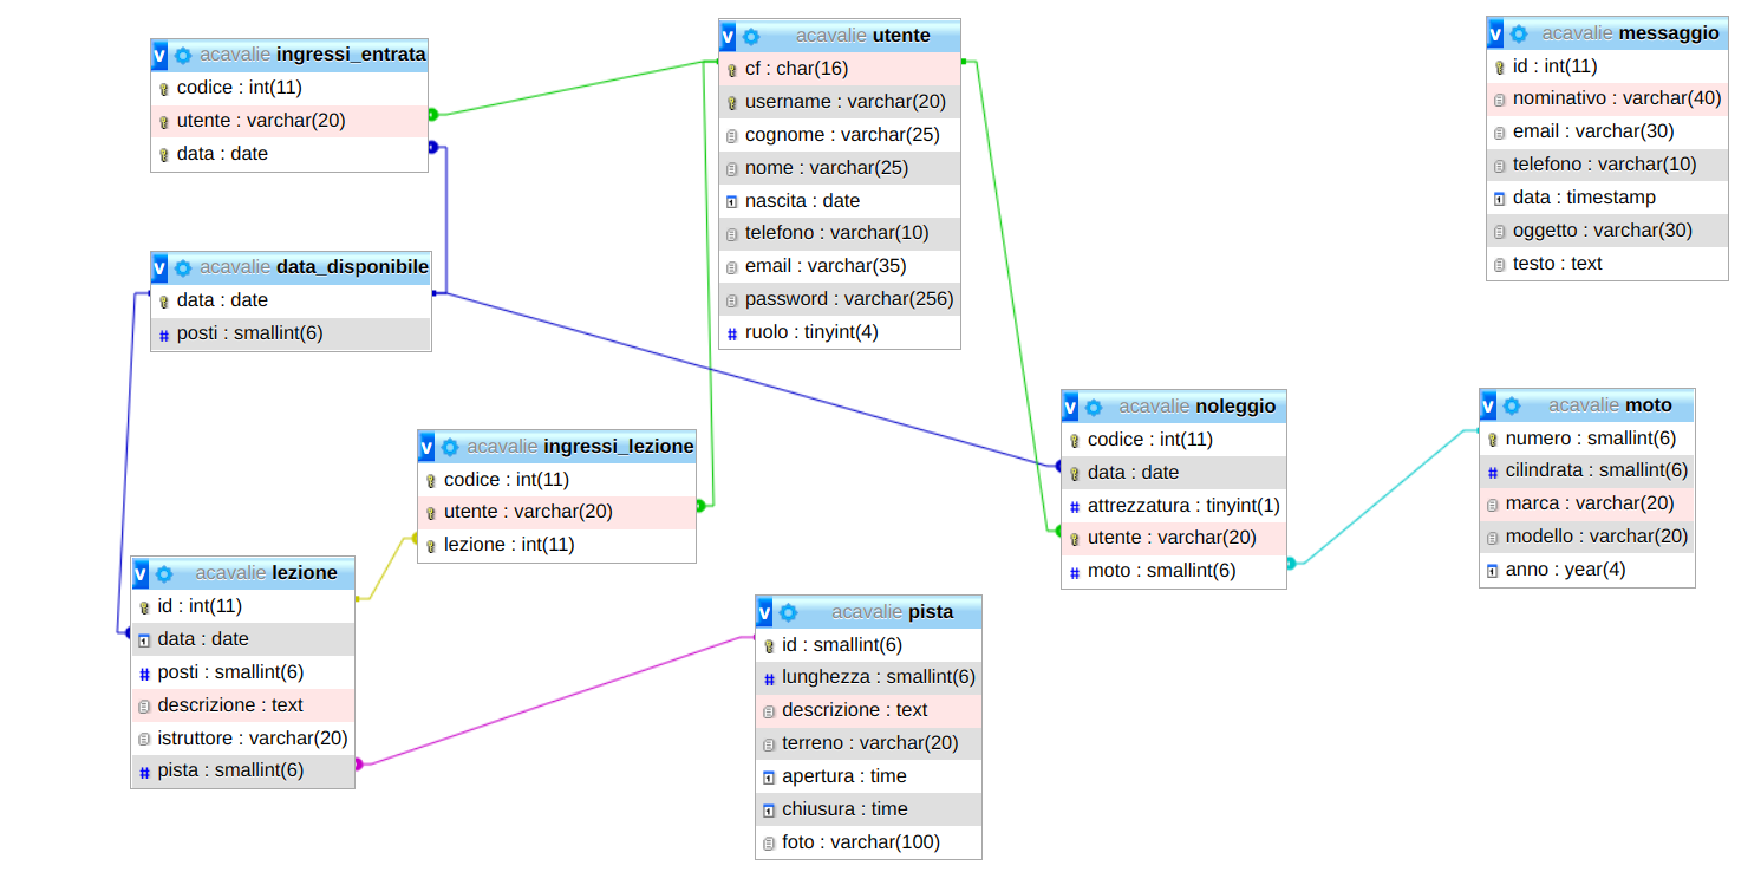
\includegraphics[scale=0.4]{./res/schemaSQL.pdf}
    \centering
    \caption{Schema SQL}
\end{figure}

			\subsubsection{JavaScript}
				Il linguaggio \textit{JavaScript} è stato utilizzato principalmente per due scopi.

Il primo riguarda la validazione dei form, i controlli sono stati fatti sia nella parte pubblica che nella parte privata (utente e admin). Per ogni pagina che necessitasse di una validazione di un form è stato creato il suo corrispondente file javascript (nomeValidation.js). Lo script analizza tutti gli input previsti per il form, controllandone la validità attraverso un'espressione regolare.
    
Il secondo, invece, è molto importante e utile per aggiornare costantemente il tipo di scelte che un utente può fare in base alle disponibilità dell'impianto. Vi sono infatti casi in cui le informazioni non possono essere rappresentate staticamente. Uno di questi casi riguarda la prenotazione di un ingresso o un corso da parte dell'utente. Viene data la possibilità all'utente di noleggiare una moto (l'attrezzatura non è un problema in questi casi) ed è quindi facile intuire che la disponibilità delle moto a noleggio varia di data in data (in base alle prenotazioni degli altri utenti).

Per poter costantemente aggiornare le moto disponibili in una giornata viene fatta una chiamata AJAX ad uno script PHP che, fornita una data di apertura, restituisce le moto ancora disponibili in quella data. Questa chiamata viene eseguita ogni volta che l'utente cambia la data in cui vuole prenotare l'ingresso o il corso.

Un altro caso simile accade nel form di prenotazione dei corsi, ma per una diversa motivazione. In questo caso si utilizza una chiamata AJAX per recuperare la descrizione del corso selezionato, evitando di costringere l'utente a muoversi tra le pagine per ricordare le informazioni del corso a cui si vuole prenotare. Questo, seppur non strettamente necessario, migliora l'esperienza utente e gli consente di portare a termine le operazioni in modo più rapido.
 
			\subsubsection{XAMPP}
				Per testare la parte dinamica del sito, in particolare le funzionalità lato server (PHP E SQL), il gruppo ha deciso di utilizzare di XAMPP. Ciò ha reso possibile
anche testare il sito con dispositivi mobili, aprendo la porta 80 del proprio pc e rendendo il tutto accessibile nella rete locale.

Tramite questo il gruppo ha potuto testare il sito provando meglio i bottoni con le proprie dita, cosa che con lo strumento di ispezione di Chrome in modalità mobile era poco affidabile.
			\subsubsection{Ispeziona di Chrome}
				La modalità ispeziona di Chrome è buona per testare CSS e HTML, in quanto permette di visionare graficamente molti
degli attributi dei fogli di stile, facilitando il debbuging. Inoltre, permette di fare cambiamenti al CSS senza intaccare i file originali,
consentendo di provare idee e metodologie di approccio di cui non si è particolarmente sicuri (come per esempio la scelta dei colori).
		\subsection{Funzionamento generale}
			Partiamo con il definire che esistono 3 categorie di utenti:
\begin{itemize}
    \item Utente generico;
    \item Utente loggato;
    \item Amministratore.
\end{itemize}

Tutte le categorie di utenti possono visualizzare la parte pubblica del sito, ovvero le disponibilità e i servizi dell'impianto. È possibile inviare una richiesta di contatto tramite l'apposito form nella pagina \textit{"Contatti"} dell'area pubblica.\\

Il servizio di prenotazione di un qualsiasi servizio richiede l'autenticazione dell'utente, il quale, se non è loggato durante la sessione, nel momento in cui clicca \textit{"Prenota Corso"} o \textit{"Prenota Ingresso"} verrà reindirizzato alla pagina
di autenticazione.
			\subsubsection{Utente Generico}
				L'utente generico è colui che deve ancora effetuare il login e dunque può navigare il sito vedendone solo la parte espositiva dello stesso.\\
Se non possiede un account, gli viene comunque fornita la possibilità di creare uno, tramite il form di registrazione, con il quale può accedere successivamente
iniziando così ad usufruire dei servizi dell'utente loggato.\\
Chiaramente, se possiede un account e vuole usufruire dei servizi dell'utente loggato,
può semplicemente fare l'accesso nell'area riservata. 
			\subsubsection{Utente Loggato}
				L'utente loggato è colui che ha effettuato l'accesso tramite le sue credenziali. Il suo stato gli permette di usare il servizio di prenotazione
del sito. In particolare può:
\begin{enumerate}
    \item \textbf{Gestire gli ingressi personali}: l'utente può prenotare un ingresso nuovo compilando l'apposito form (scegliendo data ed
    eventuali noleggi) oppure disdirne uno;
    \item \textbf{Gestire i corsi personali}: l'utente può prenotare un corso nuovo compilando l'apposito form (scegliendo data ed
    eventuali noleggi) oppure disdirne uno;
    \item \textbf{Gestire i dati personali}: può modificare i suoi dati personali (eccetto username ed e-mail).
\end{enumerate}
			\subsubsection{Amministratore}
				L'amministratore è colui che gestisce il sito e ha tutti i permessi.
In particolare può:
\begin{enumerate}
    \item \textbf{Gestire gli ingressi}: vedere le prenotazioni degli utenti, aggiungere nuove date (specificando la capacità massima), modificarle o cancellarle;
    
    \item \textbf{Gestire i noleggi}: aggiungere, togliere o modificare le moto e vedere le prenotazioni dei noleggi da parte degli utenti;
    
    \item \textbf{Gestire i tracciati}: aggiungere, togliere o modificare i tracciati;
    
    \item \textbf{Gestire i corsi}: aggiungere, togliere o modificare i corsi e vedere le prenotazioni da parte degli utenti;
    
    \item \textbf{Gestire i dati personali}: modificare i suoi dati personali (eccetto username ed e-mail);
    
    \item \textbf{Promuovere l'utenza}: promuove gli utenti ad admin (l'impianto assume constantemente personale);
    
    \item \textbf{Visualizzare i messaggi}: visualizzare i messaggi che arrivano dal form di contatto.
\end{enumerate}
		\subsection{Intrusività}
			Di seguito verrà descritto il livello di intrusività dei linguaggi rispetto al codice sorgente HTML:
\begin{itemize}
    \item \textbf{CSS}: \underline{non} intrusivo. Tutto il codice CSS è stato inserito in un file a parte, evitando del tutto pratiche come il
    CSS inline o embedded.
    \item \textbf{PHP}: \underline{non} intrusivo. Sebbene ci sia del codice HTML all'interno di alcuni file PHP, la corrispondente
    pagina HTML non contiene codice PHP. La motivazione per la quale c'è del codice HTML in file PHP è che spesso i dati, essendo molto dinamici,
    cambiano spesso in base sia all'input dell'utente che dell'amministratore. Dunque in base alla presenza o meno di alcuni di questi 
    (per esempio le date d'ingresso) possono comparire o meno determinati elementi HTML.
    \item \textbf{Javascript}: \underline{non} intrusivo. Tutto il codice javascript è stato inserito in un file a parte.
\end{itemize}
		
	\newpage

	\section{Validazione}
		La validazione delle pagine è fondamentale per garantire un sito web accessibile e aderente agli standard. In particolare sono stati utilizzati i seguenti strumenti per la validazione automatica del sito. % anche vuoto
		\subsection{Strumenti usati}
			Per la validazione dei file HTML è stato usato il validatore di W3C\footnote{https://validator.w3.org/}.
Per il CSS del sito è stato usato il validatore CSS\footnote{http://www.css-validator.org/} sempre offerto dal W3C.
L'accessibilità è stata controllata tramite lo strumento WAVE Evaluation\footnote{https://wave.webaim.org/}.
Infine, per il PHP ed il Javascript, anche se non richiesto, abbiamo utilizzato rispettivamente PhpCodeChecker\footnote{https://phpcodechecker.com/} ed Esprima\footnote{https://esprima.org/demo/validate.html}.
			\subsubsection{WAVE Evaluetion}
				Questo tool ha permesso al gruppo di trovare alcuni problemi legati all'accessibilità dei contenuti. Esso ha individuato alcune problematiche rispetto al tipo di attributi \textit{aria} utilizzati e rispetto alla lunghezza dell'\textit{alt} di alcune immagini. Sebbene abbia individuato dei falsi negativi è stato utile per raffinare alcuni aspetti dell'accessibilità. È stato utilizzato anche per i test sul contrasto dei colori utilizzati.
			\subsubsection{W3C HTML Validator}
				Lo strumento di validazione di W3C ci ha consentito di validare anche l’HTML prodotto dalle pagine PHP, poichè permette di incollare direttamente il codice HTML prodotto dallo script. È il motivo per cui è stato utilizzato per validare tutto il codice HTML. 

Non è stato possibile testare tutte le possibili combinazioni degli esiti degli script PHP (richiedeva la presenza di situazioni complesse da simulare). Per questo motivo, oltre al tool indicato, è stata effettuata la verifica manuale in stile \textit{walkthrough} degli script PHP, controllando che tutti i testi aggiunti dinamicamente venissero inclusi nei corretti tag.
			\subsubsection{W3C CSS Validator}
				Abbiamo utilizzato anche il servizio di validazione del CSS del W3C così da assicurarci il rispetto il più rigorosamente possibile dello standard.
			\subsubsection{PhpCodeChecker}
				Attraverso l’utilizzo di questo tool è stata verificata la sintassi di tutti i file PHP. È stato molto utile in quanto essendo il sito molto
dinamico buona parte del sito web è scritta con questo linguaggio.
			\subsubsection{Esprima}
				Tramite l’utilizzo di questo strumento è stata controllata la sintassi ditutti gli script javascript utilizzati, come la validazione dei campi
lato client o le chiamate HTTP AJAX.
				
	\newpage

	\section{Organizzazione del lavoro}
		Il lavoro del progetto \textit{Adrenaline Motocross Park} è stato suddiviso nel seguente modo:
\begin{itemize}
    \item Brugnolaro Filippo:
        \begin{itemize}
            \item[$\circ$] Parte dei file HTML della parte pubblica
            \item[$\circ$] Maggior parte dei file Javascript
            \item[$\circ$] Validazione HTML e Javascript
            \item[$\circ$] Prova con screen reader
            \item[$\circ$] Stesura della relazione
        \end{itemize}
    \item Cavaliere Alessandro:
        \begin{itemize}
            \item[$\circ$] File HTML della parte privata dell'amministratore
            \item[$\circ$] Maggior parte dei file PHP della parte privata dell'amministratore
            \item[$\circ$] Parte dei file Javascript
            \item[$\circ$] Parte del database SQL
            \item[$\circ$] Parte dei file CSS
        \end{itemize}
    \item Gambirasio Leonardo:
        \begin{itemize}
            \item[$\circ$] Parte dei file HTML della parte pubblica
            \item[$\circ$] Parte dei file PHP
            \item[$\circ$] Parte dei file CSS
            \item[$\circ$] Validazione CSS
            \item[$\circ$] Test dei browser
        \end{itemize}
    \item Simionato Riccardo:
        \begin{itemize}
            \item[$\circ$] File HTML della parte priva dell'utente
            \item[$\circ$] Maggior parte dei file PHP della parte privata dell'utente
            \item[$\circ$] Parte del database SQL
            \item[$\circ$] Parte dei file CSS
            \item[$\circ$] Validazione dei file PHP
        \end{itemize}
\end{itemize}
	
	\newpage
	
	\appendix
	\addcontentsline{toc}{part}{Appendice}
	\section{Note per la correzione}
		In questa sezione vengono illustrate alcune informazioni utili per i valutatori.
		\subsection{Credenziali}
			Vengono fornite le credenziali dell’account amministratore:
\begin{itemize}
    \item Username: \textit{admin}
    \item Password: \textit{admin}
\end{itemize}
Vengono fornite le credenziali dell’account utente:
\begin{itemize}
    \item Username: \textit{user}
    \item Password: \textit{user}
\end{itemize}
É in ogni caso sempre possibile creare nuovi utenti tramite l'apposito form di registrazione.
		\subsection{Popolamento}
			Per avere una reale presentazione del sito, sono già stati inseriti alcuni record: date di apertura, corsi, tracciati moto noleggiabili, prenotazioni ingressi/corsi, messaggi.\\
I dati inseriti non devono per forza corrispondere con la realtà e per tanto non devono essere considerati come difetti del sito.
		\subsection{Visibilità}
			A causa dell'utilizzo di icone soggette a copyright che ne permette l'uso esclusivamente personale, il sito non può essere in alcun modo
visibile al pubblico.

    
\end{document}